\section{Korištene tehnologije}

\subsection{ASP.NET Core}

ASP.NET Core (engl. \textit{Active Server Pages Network Enabled Technologies Core}) višeplatformski je okvir otvorenog k\^oda korišten za izradu aplikacija. Inačica je ASP.NET okvira opće namjene koja se može koristiti na operacijskim sustavima Windows, Linux, macOS te Dockeru. ASP.NET Core stvoren je uzevši najkorisnije značajke .NET-a i .NET Corea. Pomoću okvira ASP.NET Core omogućena je izrada aplikacija za bilo koji tehnološki uređaj kao što su iOS uređaji, Android uređaji, oblak i drugi. ASP.NET Core u \textit{namespaceu} \texttt{Microsoft.AspNetCore.Authorization} sadrži tipove koji omogućuju autorizaciju\cite{aspNetCore}.


\subsubsection{C\#}
C\# je objektno-orijentiran programski jezik čija se popularnost povećala pojavom okvira .NET. Svrha C\#-a jest da bude jednostavan i moderan programski jezik dobiven kombinacijom elemenata jezika C i C++  s utjecajem jezika Java te time postaje robustan jezik za razvoj \textit{softvera}. Uveden je i koncept alata LINQ (engl. \textit{Language Integrated Query}) za postavljanje upita i manipuliranje podatcima iz baze podataka i drugih izvora. Omogućeno je korištenje asinkronih metoda (pogledati poglavlje~\ref{subsec:repo}) uz pomoć ključnih riječi \texttt{async} i \texttt{await} kojima se omogućuje izvršavanje zadataka bez blokiranja glavne niti. Jezik C\# podržava i automatsko upravljanje memorijom (engl. \textit{auto-garbage collection}). Uz prethodno navedene, neke od glavnih karakteristika C\#-a su višenitnost (engl. \textit{multithreading}) i stroga tipizacija koja zahtijeva određivanje tipova podataka tijekom kompajliranja~\cite{cSharp}.

\subsubsection{Upravitelj paketa NuGet}
NuGet (engl. \textit{NuGet Package Manager}) alat je za upravljanje paketa u ASP.NET okviru. Korišten je za instalaciju paketa (biblioteka) koji su potrebni pri izradi aplikacije. Pakete je moguće izraditi pomoću aplikacije NuGet i pohraniti ih u privatni ili javni repozitorij kao ZIP datoteke s ekstenzijom \texttt{.nupack} ili \texttt{.nupkg}\cite{nuGet}.
\begin{figure}[H]
	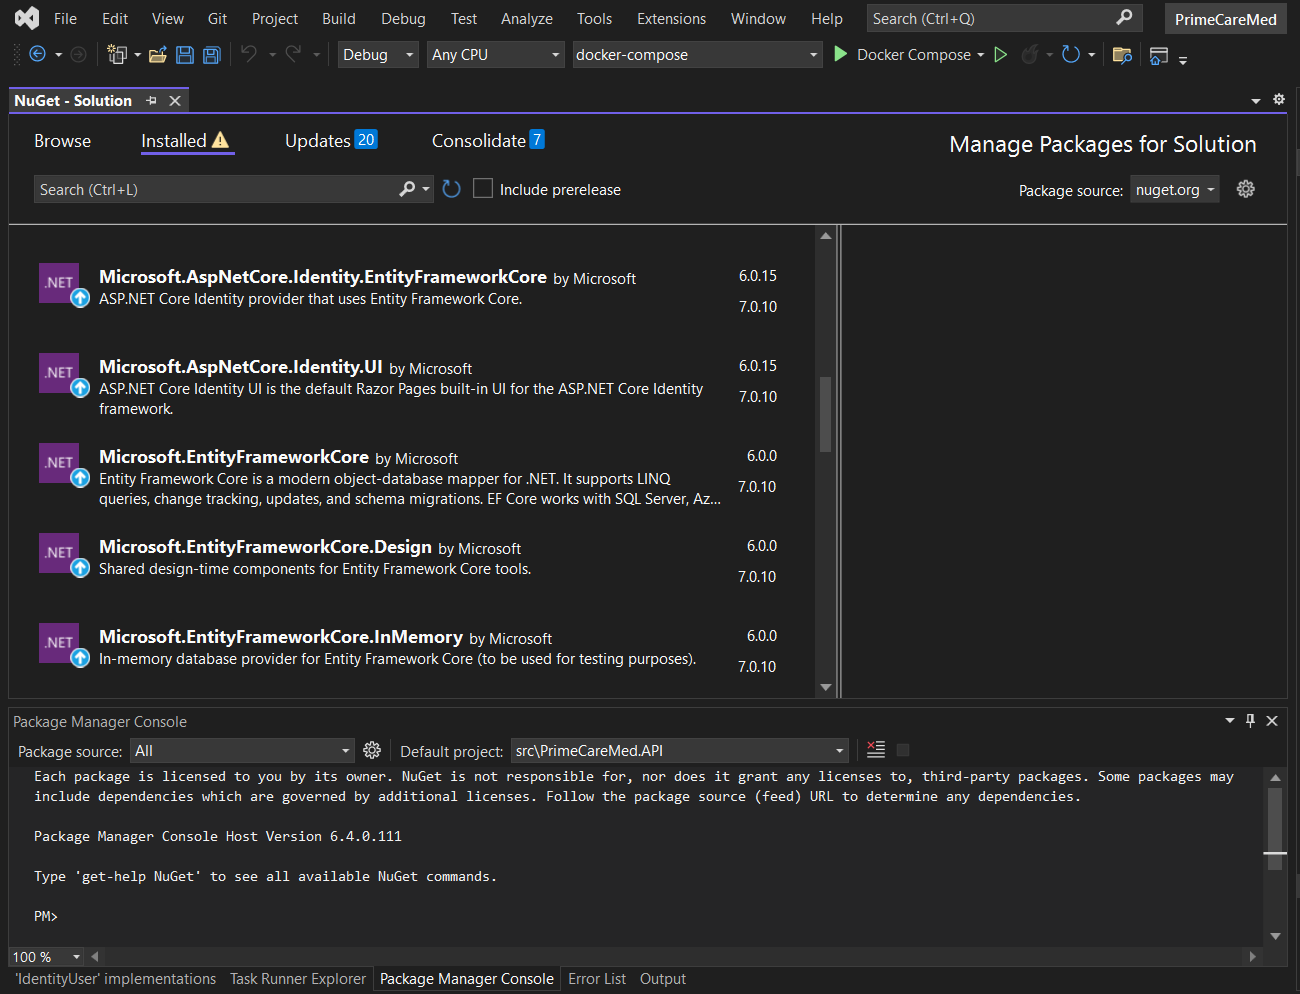
\includegraphics[width=1\linewidth,clip=]{assets/NuGet.png}
	\centering
	\caption{NuGet Package Manager i Package Manager Console}
	\label{fig:appDir}
\end{figure} 
 
\subsubsection{Entity Framework Core} 
 
 Entity Framework Core višeplatformska je biblioteka otvorenog k\^oda koja omogućuje pristup bazi podataka preko izvornog k\^oda pomoću ORM-a (\textit{Object-relational mapping})\cite{entityFrameworkCore}. Entity Framework Core radi na operacijskim sustavima Windows, MacOS i Linux a omogućen je instalacijom paketa NuGet u aplikaciji pomoću upravitelja paketa (engl. \textit{Package Manager}) ili .NET sučelja naredbenog retka (engl.\textit{Command Line Interface}) naredbom prikazanom u ispisu~\ref{lst:nuGetAdd}.
\begin{lstlisting}[caption={Naredba za dodavanje NuGet paketa}, label=lst:nuGetAdd]
dotnet add [<PROJECT>] package <PACKAGE_NAME>
    [-f|--framework <FRAMEWORK>] [--interactive]
    [-n|--no-restore] [--package-directory <PACKAGE_DIRECTORY>]
    [--prerelease] [-s|--source <SOURCE>] [-v|--version <VERSION>]
\end{lstlisting}
 
\subsubsection{Razor Pages}
Razor Pages model je za programiranje web aplikacija koji omogućuje jednostavno učitavanje podataka. Sintaksno je i funkcionalno sličan modelu MVC \\(\textit{Model-View-Controller}). Najvažnija značajka kojom se model Razor Pages razlikuje od modela MVC su datoteka \texttt{.cshtml} te datoteka \texttt{.cshtml.cs} takozvanog k\^oda iza (engl. \textit{code-behind}) koje su omogućile neupotrebu odvojenih datoteka za modele i upravljače (engl. \textit{controller}). Stranica upravlja vlastitim modelom koji se definira u code-behind datoteci\cite{RazorPages}. Primjer upravljanja modelom bit će prikazan u poglavlju \ref{subsec:izvedbaRP}.

\subsubsection{ASP.NET Core Identity}
\label{subsubsec:IdentityCore}
 
ASP.NET Core Identity dostupan je kao biblioteka Razor Class omogućena instalacijom paketa NuGet.  ASP.NET Core Identity podržava funkcionalnosti za upravljanje korisničkog sučelja, lozinki, uloga korisnika, potvrdu mail računa i drugih značajki korisnika aplikacije. Izvorni k\^od dostupan je na platformi GitHub \cite{aspNETGitHub}. U aplikaciji \textit{PrimeCareMed}, instalirani su paketi NuGet:\\\texttt{Microsoft.AspNetCore.Identity.EntityFrameworkCore} \\ \texttt{Microsoft.AspNetCore.Identity.UI}  \\ čime je omogućeno korištenje klase \texttt{IdentityUser} u svrhu naslijeđa od strane klase \texttt{ApplicationUser}. Uz nasljeđivanje klase \texttt{IdentityUser}, potrebno je naslijediti \texttt{IdentityDbContext} tipa \texttt{ApplicationUser} prikazano na ispisu~\ref{inheritIdentity}.
\begin{lstlisting}[caption={Nasljeđivanje klase \texttt{IdentityDbContext}}, label=inheritIdentity]
public class DatabaseContext : IdentityDbContext<ApplicationUser>
\end{lstlisting}

\begin{figure}[H]
	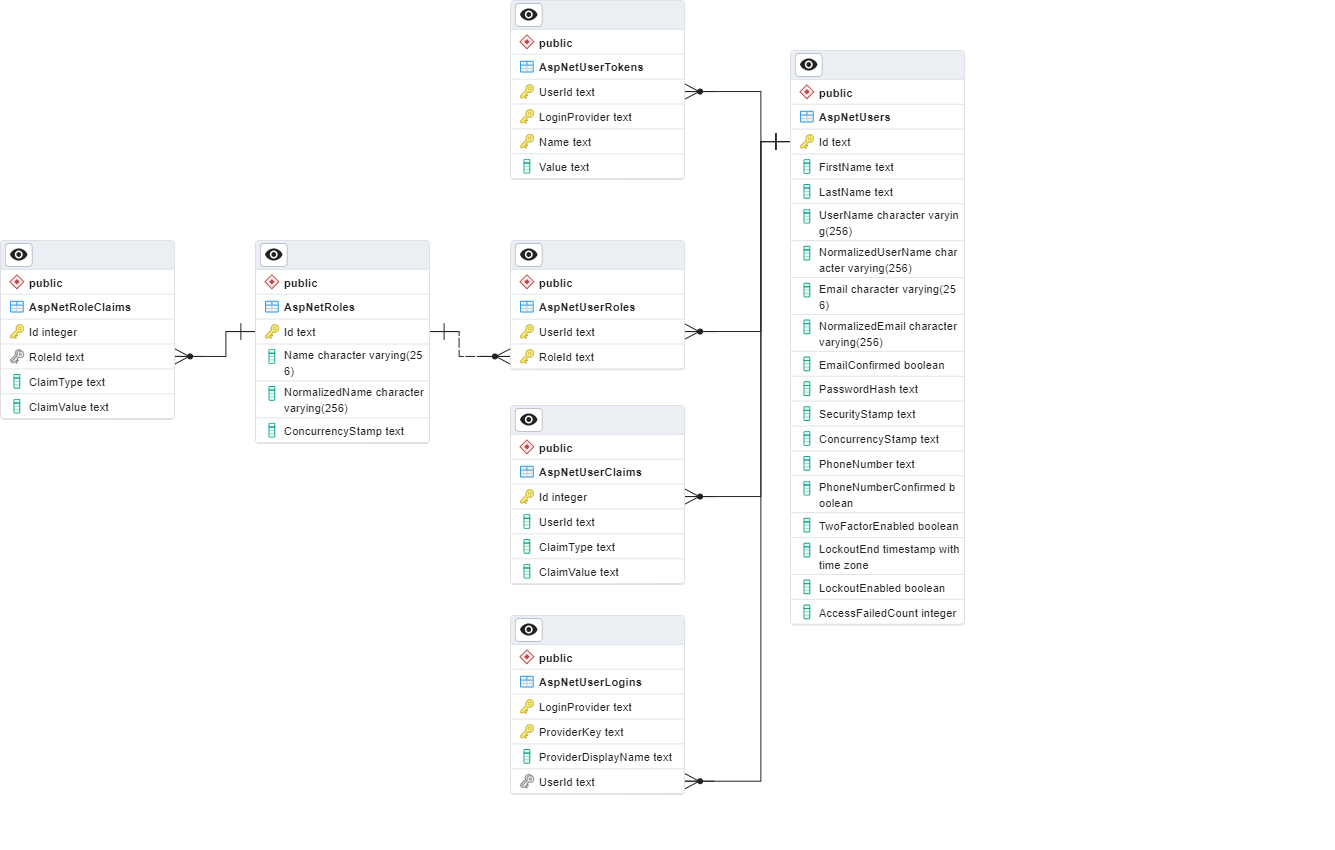
\includegraphics[width=1\linewidth,clip=]{assets/IdentityDatabase.png}
	\centering
	\caption{Baza podataka nakon nasljeđivanja klase \texttt{IdentityUser}}
	\label{fig:IdentityDatabase}
\end{figure}


\paragraph{Scaffold Identity}\mbox{}\\
\indent Desnim klikom na \texttt{PrimeCareMed.Frontend} > \texttt{Add} > \\\texttt{New Scaffolded Item} otvara se prozor prikazan na slici~\ref{fig:identityScaffold} te je omogućeno dodavanje opcije \texttt{Identity}. Dodavanjem Identity Scaffoldera na projekt \\\texttt{PrimeCareMed.Frontend} dobivene su unaprijed kreirane stranice Razor koje omogućuju funkcionalnosti povezane s upravljanjem korisničkih računa\cite{scaffoldIdentity}.
\begin{figure}[H]
	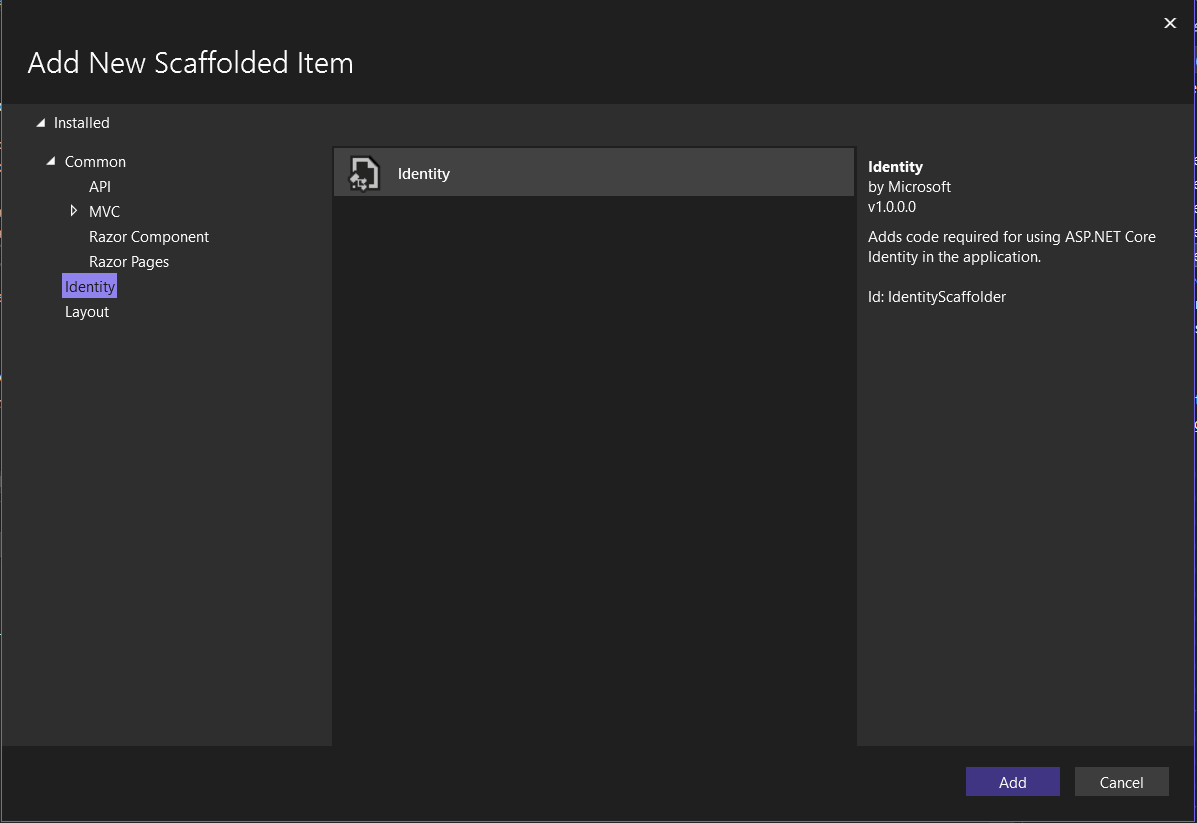
\includegraphics[width=0.8\linewidth,clip=]{assets/identityScaffold.png}
	\centering
	\caption{Identity Scaffolded Item}
	\label{fig:identityScaffold}
\end{figure}
\subsection{Docker}

Kao razvojno okruženje, u svrhu izvođenja web aplikacije na različitim operativnim sustavima korišteni su Docker spremnici (engl. \textit{containers}). Prilikom stvaranja projekta \texttt{PrimeCareMed.Frontend}, odabrana je opcija Enable Docker prikazana na slici~\ref{fig:enableDocker}. Na postojeći projekt \texttt{PrimeCareMed.API} Docker podrška omogućena je dodavanjem opcije \textit{Docker Support} prikazane na slici~\ref{fig:addDocker}\cite{containerToolsDocker} \cite{multiContainerDocker}.

\begin{figure}[H]
	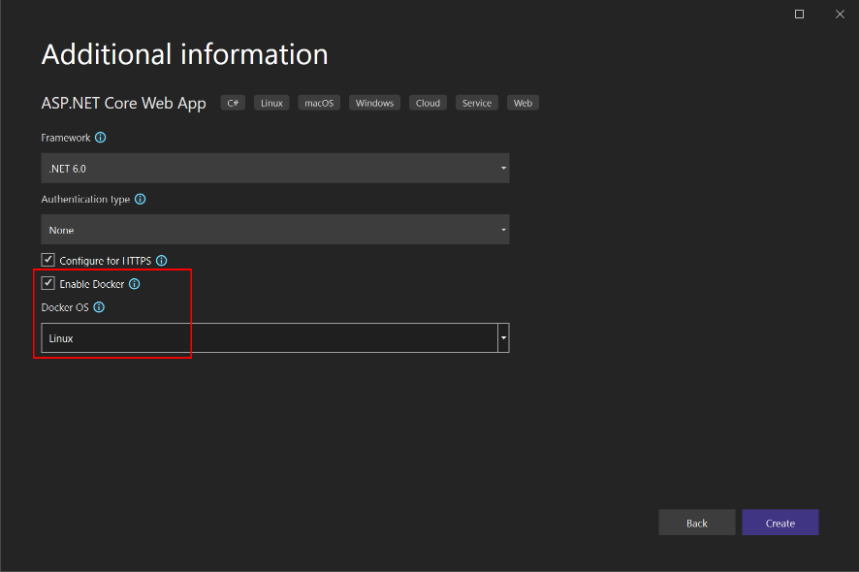
\includegraphics[width=0.6\linewidth,clip=]{assets/enableDocker.png}
	\centering
	\caption{Uključivanje Docker podrške prilikom kreiranja projekta}
	\label{fig:enableDocker}
\end{figure}

\begin{figure}[H]
	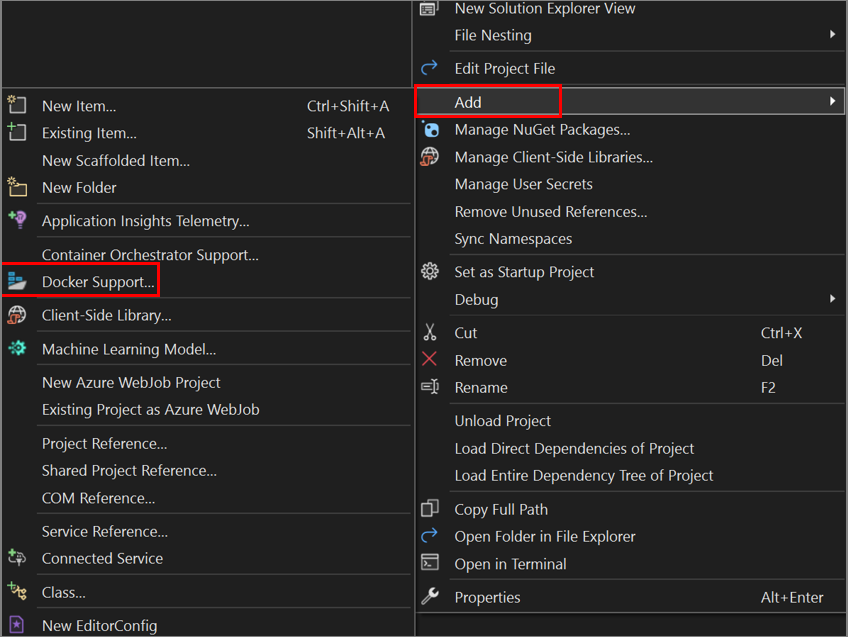
\includegraphics[width=0.6\linewidth,clip=]{assets/addDockerSupport.png}
	\centering
	\caption{Uključivanje Docker podrške na postojeći projekt}
	\label{fig:addDocker}
\end{figure}

Odabirom opcije \textit{Container Orchestrator Support} sa slike~\ref{fig:addDocker} stvara se zaseban projekt unutar \textit{solutiona} naziva \texttt{docker-compose} koji sadrži datoteke \texttt{.dockerignore},\\ \texttt{docker-compose.yml} i \texttt{launchSettings.json} vidljive na slici~\ref{fig:dockerCompose} dok se datoteke naziva \texttt{Dockerfile} nalaze u pripadajućim projektima: \texttt{PrimeCareMed.Frontend} i \texttt{PrimeCareMed.API}.

\begin{figure}[H]
	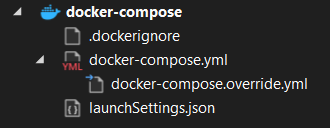
\includegraphics[width=0.6\linewidth,clip=]{assets/dockerCompose.png}
	\centering
	\caption{Projekt \texttt{docker-compose}}
	\label{fig:dockerCompose}
\end{figure}

U ispisu~\ref{ymlDatoteka} prikazani su docker servisi u datoteci \texttt{docker-compose.yml} koji predstavljaju spremnike u aplikaciji Docker Desktop koji će biti pokrenuti prilikom pokretanja aplikacije (pogledati sliku~\ref{fig:dockerDesktop}).
\begin{lstlisting}[caption={Datoteka \texttt{docker-compose.yml}}, label=ymlDatoteka]
version: '3.4'

services:
    
  primecaremed.frontend:
    image: ${DOCKER_REGISTRY-}primecaremedfrontend
    build:
      context: .
      dockerfile: src/PrimeCareMed.Frontend/Dockerfile
    environment:
      CONNECTION_STRING: "Host=postgres;Port=5432;Database=postgres;Username=admin;Password=root;Integrated Security=true;Pooling=true;"

  primecaremed.api:
    image: ${DOCKER_REGISTRY-}primecaremedapi
    build:
      context: .
      dockerfile: src/PrimeCareMed.API/Dockerfile
    environment:
       CONNECTION_STRING: "Host=postgres;Port=5432;Database=postgres;Username=admin;Password=root;Integrated Security=true;Pooling=true;"

  postgres:
    image: postgres:alpine
    environment:
      POSTGRES_DB: postgres
      POSTGRES_USER: admin
      POSTGRES_PASSWORD: root
    ports:
      - 5432:5432
    volumes:
      - postgres-data:/var/lib/postgresql/data
    restart: unless-stopped

  pgadmin4:
    image: dcagatay/pwless-pgadmin4:latest
    depends_on:
      - postgres
    ports:
      - 15432:80
    environment:
      POSTGRES_USER: admin
      POSTGRES_PASSWORD: root
    restart: unless-stopped
    
  mailhog:
    image: mailhog/mailhog
    ports:
      - '1025:1025' # smtp server
      - '8025:8025' # web ui

volumes:
  postgres-data:

\end{lstlisting}

U ispisu~\ref{dockerfileDatoteka} prikazana je datoteka \texttt{Dockerfile} u kojoj se stvara datoteka\\\texttt{PrimeCareMed.Frontend.dll} (\textit{DLL - Dynamic-link library}) koja sadrži izvršni k\^od.

\begin{lstlisting}[caption={Datoteka \texttt{Dockerfile} u projektu \texttt{PrimeCareMed.Frontend}}, label=dockerfileDatoteka]
FROM mcr.microsoft.com/dotnet/aspnet:6.0 AS base
WORKDIR /app
EXPOSE 80
EXPOSE 443

FROM mcr.microsoft.com/dotnet/sdk:6.0 AS build
WORKDIR /src
COPY ["src/PrimeCareMed.Frontend/PrimeCareMed.Frontend.csproj", "src/PrimeCareMed.Frontend/"]
RUN dotnet restore "src/PrimeCareMed.Frontend/PrimeCareMed.Frontend.csproj"
COPY . .
WORKDIR "/src/src/PrimeCareMed.Frontend"
RUN dotnet build "PrimeCareMed.Frontend.csproj" -c Release -o /app/build

FROM build AS publish
RUN dotnet publish "PrimeCareMed.Frontend.csproj" -c Release -o /app/publish /p:UseAppHost=false

FROM base AS final
WORKDIR /app
COPY --from=publish /app/publish .
ENTRYPOINT ["dotnet", "PrimeCareMed.Frontend.dll"]
\end{lstlisting}

\begin{figure}[H]
	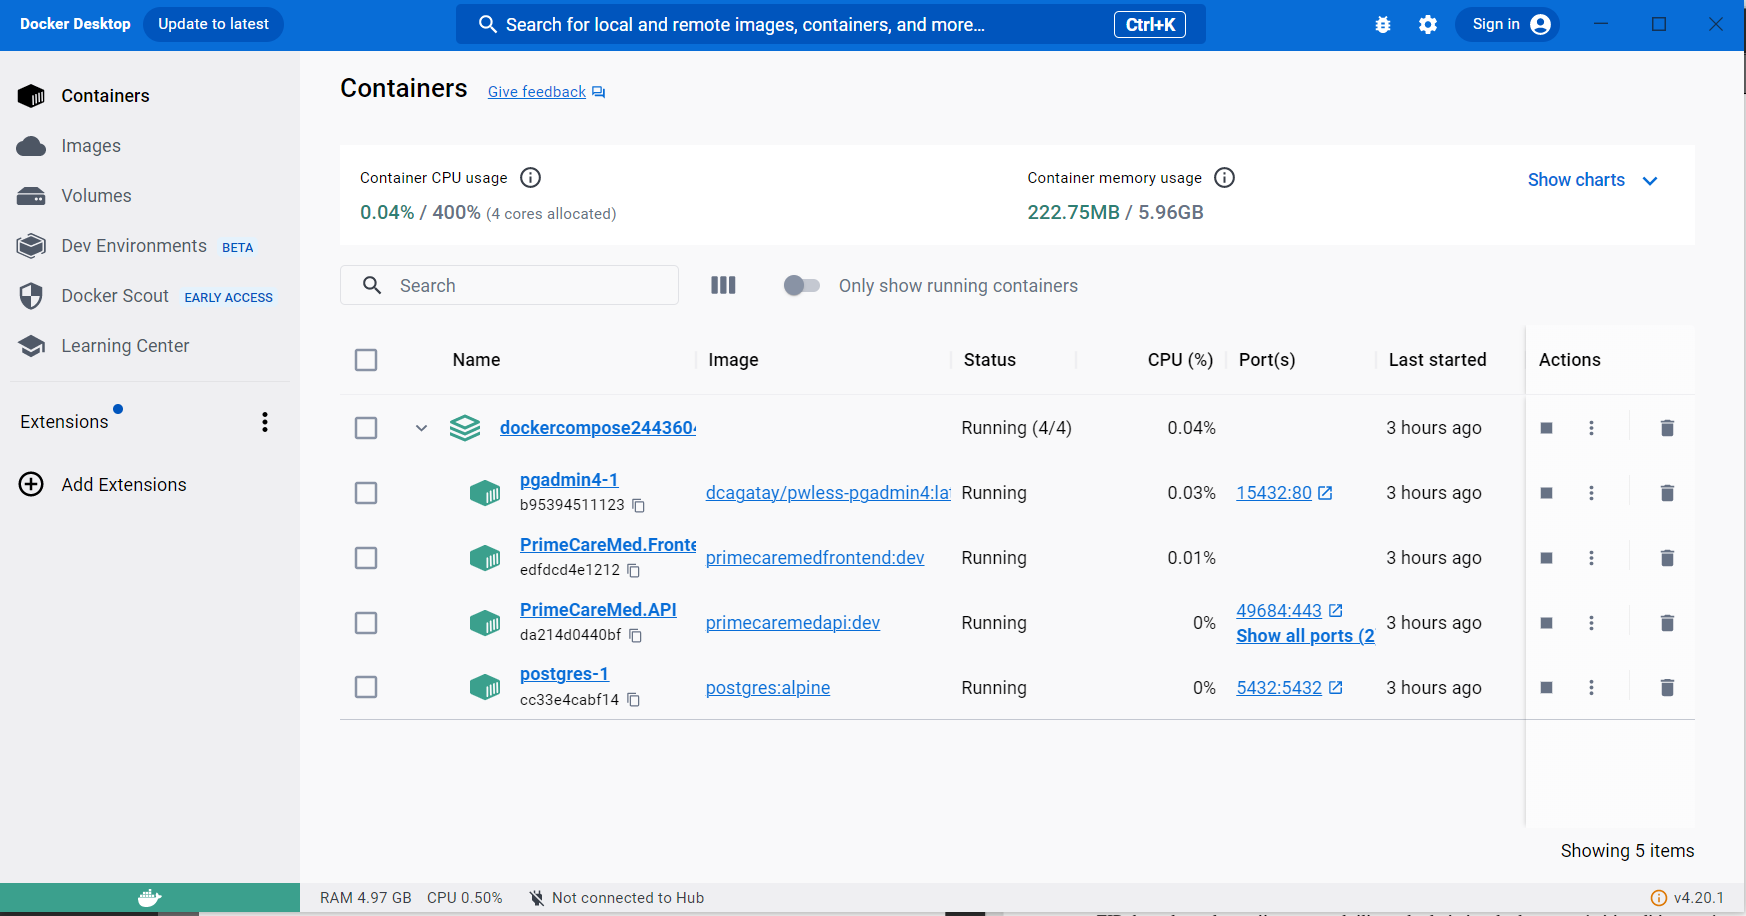
\includegraphics[width=0.8\linewidth,clip=]{assets/dockerDesktop.png}
	\centering
	\caption{Pokrenuti spremnici u aplikaciji Docker Desktop}
	\label{fig:dockerDesktop}
\end{figure}


\subsection{PostgreSQL}
PostgreSQL besplatan je program otvorenog k\^oda za upravljanje objektno-relacijskim bazama podataka (engl. \textit{ORDBMS - Object-Relational Database Management System}) koristeći jezik SQL (\textit{Structured Query Language}). Dozvoljena su proširenja mogućnosti PostgreSQLa kao što su dodavanje novih tipova podataka, operatora ili funkcija\cite{PostgreSQL}. PostgreSQL trenutno je jedna od najnaprednijih baza podataka otvorenog k\^oda. Prikaz sheme baze podataka, strukture svih entiteta i druge mogućnosti PostgreSQLa dostupne su u sučelju pgAdmin.

